\chapter{Introduction}
\label{chapter:introduction}

% Describe Distributed Safety-critical real-time systems
Safety and mission-critical distributed real-time embedded (DRE) systems are increasingly being used in a variety of domains such as avionics \cite{burke2010distributed}, locomotive control \cite{zimmermann2003train}, and industrial control systems \cite{zoitl2008real}.  
% Describe Component-based DRE systems - Trends
Given the dominant role of software in such systems, growing both in size and complexity, utilizing predictable and dependable software is critical for system safety. To mitigate this complexity, model-driven, component-based software engineering (CBSE) and development \cite{beydeda2005model, heineman2001component, clemens1998component} has become an accepted practice. CBSE tackles the increased demands with respect to requirements engineering, high-level design, design error detection, tool integration, verification and maintenance. The widespread use of component technology in the market has made CBSE a focused field of research in the academic sectors. Applications are built by assembling together small, tested component building blocks that implement a set of services. These building blocks are typically built from class models, or imported from other projects/vendors and connected together via exposed interfaces, providing a "black box" approach to software construction. Component models describe the software components that are used to build the system. The reusable nature of components leads to developers focusing on other critical parts of the system design, leading to shorter development cycles and reduced costs. 

Complex, managed systems, e.g. a fractionated spacecraft following a mission
timeline and hosting distributed software applications expose heterogeneous concerns such as strict timing requirements, complexity in deployment, repair and integration; and resilience to faults. High-security and time-critical software applications hosted on such platforms run concurrently with all of the system-level mission management and failure recovery tasks that are periodically undertaken on the distributed nodes. Once deployed, it is often difficult to obtain low-level access to such remote systems for run-time debugging and evaluation. These types of systems therefore demand advanced design-time modeling and analysis methods to detect possible anomalies in system behavior, such as unacceptable response times, before deployment.

Our team has designed and prototyped a full information architecture called \textbf{D}istributed \textbf{RE}al-time \textbf{M}anaged \textbf{S}ystem (DREMS) \cite{ISIS_F6_Aerospace:12,DREMS13Software} that addresses requirements for rapid component-based application development. In prior work, we have described the design-time modeling capability \cite{ISIS_F6_SFFMT:13}, and the component model used to build and execute applications \cite{ISIS_F6_ISORC:13}.
%This architecture consists of a design-time tool suite for modeling, analysis, synthesis, integration, debugging, testing, and maintenance of application software built from reusable components. The architecture also provides a run-time software platform for deploying, managing, and executing application software on a network of mobile computing nodes. 
The formal modeling and analysis method presented in this paper focuses on applications that rely on this foundational architecture. The principle behind design-time analysis here is to map the structural and behavioral specifications of the system under analysis into a formal domain for which analysis tools exist. The key is to use an appropriate model-based abstraction such that the mapping from one domain to another remains valid under successive refinements in system development such as code generation. 
%This abstraction includes formalizing (1) the structure of component building blocks, (2) the semantics of component interaction patterns, and (3) the abstract temporal behavior of application components. 
The analysis must ensure that as long as the assumptions made about the system hold, the behavior of the system lies within the safe regions of operation.  The results of this analysis will enable system refinement and re-design if required, before actual code development. 

%\AD{Suggested Problem Statement: The principle behind design time analysis is to map the model of the system under analysis into a formal domain for which analysis tools exist. Key here is to use appropriate model based abstraction such that the mapping from one domain to other domain remains valid under successive refinements such as code-generation. For our work, we have chose the colored petri net as the formal domain - please describe why. }

Figure \ref{fig:sdlc} shows a \emph{spiral model} \cite{boehm1988spiral} of a typical industrial software/system development life cycle.  The five primary stages in this loop are: (1) Requirements analysis, (2) software design, (3) implementation, (4) integration (5) testing and debugging, (6) design evolution. Any system design first begins with an informal description of the requirements. Analyzing the requirements yields the necessary layers of software (or hardware) required in the system design. Once the design is complete, the pieces/layers of software are implemented by software developers. These pieces of software i.e. components are then \emph{integrated} together to obtain the overall system.  A separate team of testers check the integrated system using various testing methods including unit tests and integration tests. Once the software has met certain testing requirements, the software becomes more robust. Inconsistencies identified during this testing process often causes changes to high-level requirements. This cycle repeats as long as the software is \emph{alive}. Any new features to be integrated in this system need to go through these steps. 

\begin{figure}[h]
	\centering
	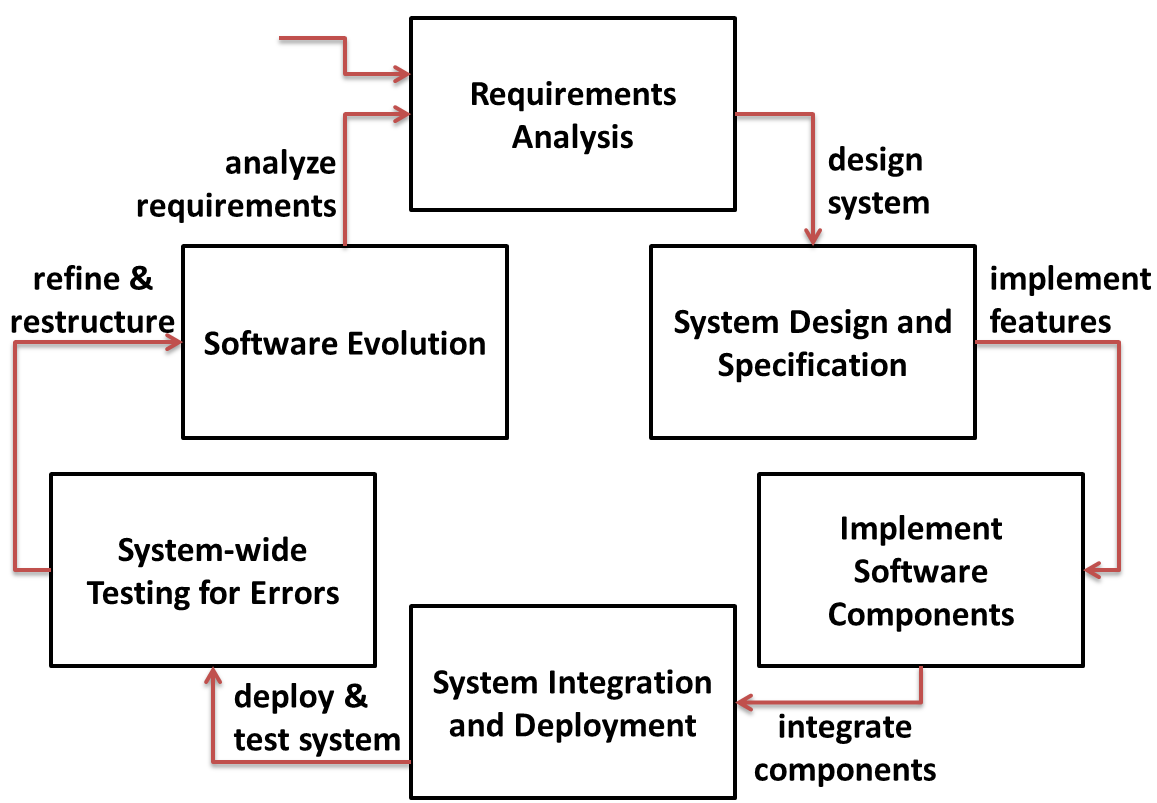
\includegraphics[width=0.9\textwidth]{./figs/sdlc}
	\caption{Industrial Software/System Development Life Cycle}
	\label{fig:sdlc}
\end{figure}

The analysis work proposed in this thesis supports a verification-driven workflow for component-based software development, as shown in Figure \ref{fig:big_picture}. Application developers use domain-specific modeling languages to model the component assembly, interaction patterns, component execution code, sequence of operations, and associated temporal properties such as estimated execution times, deadlines etc. Using such application-specific parameters in the \textit{design} model, a Colored Petri net-based (CPN) \cite{CPN} \textit{formal analysis model} is generated. The system behavior is both simulated and analyzed using a CPN execution engine, CPN Tools \cite{CPNTools}, and useful properties of the system are verified. By generating a bounded \emph{state space} of the system, the execution traces exhibited by the system are searched for property violations. Such system properties include the lack of deadlocks, deadline violations and worst-case trigger-to-response times. The goal of this analysis is to ensure that a component-based system, an assembly of tested component building blocks, meets the temporal specifications and requirements of the system.  

\begin{figure}[h]
	\centering
	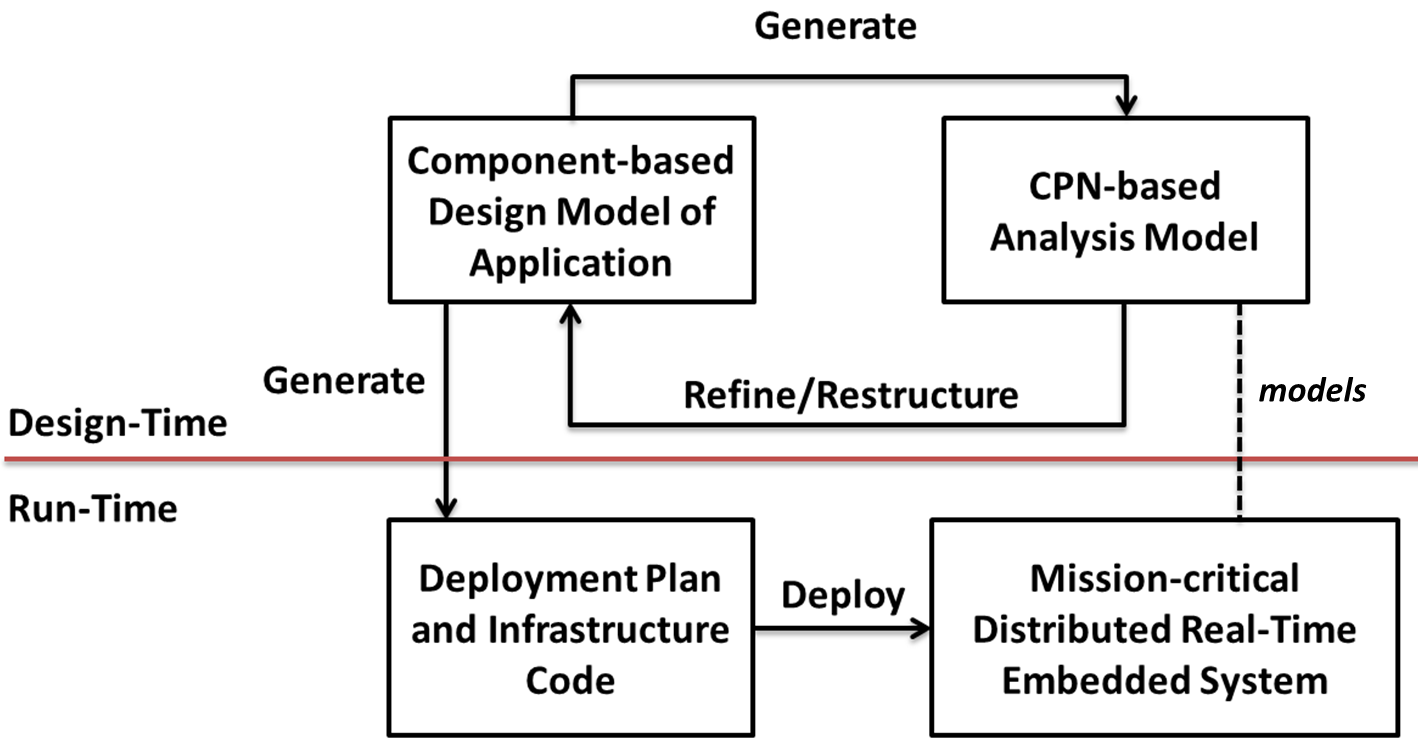
\includegraphics[width=0.9\textwidth]{./figs/big_picture}
	\caption{Verification-driven Workflow}
	\label{fig:big_picture}
\end{figure}

The results of this analysis help improve the structure of the application, enabling safe deployment of dependable components that are known to operate within system specifications. Some implicit assumptions to this analysis include a prior knowledge of WCET estimates for the various code blocks in the component execution code. When designing the overall system, the analysis can be performed by assigning \emph{time budgets} to the discrete tasks in the execution. This enables timing analysis before implementation and also uses the time budgets as requirements for efficient code implementation. These budgets are often derived from high-level requirements and appropriately distributed between the different components in the system. The analyzed system may not necessary be complete, but instead be in a process of evolution. As the design progresses, the system requirements become extended and the design is re-verified at each stage to ensure the timing guarantees advertised. 

The remainder of this proposal is organized as follows. Chapter II describes some fundamental concepts about distributed real-time systems, component-based software and some challenges in timing analysis. Chapter III describes the related research in timing analysis and verification for distributed real-time embedded applications. Chapter IV introduces the DREMS infrastructure and Component Model used to experiment with and validate the timing analysis results. This chapter also proposes the Colored Petri net-based timing analysis methodology devised for component-based DRE systems, including published results and proposed contributions. Chapter V concludes the proposal, providing a tentative timetable for the successful completion of the proposed work. Finally, Chapter VI lists relevant publications.





